% !TeX program = pdflatex
\documentclass[11pt]{article}
\usepackage{graphicx}
\usepackage[margin=28mm]{geometry}
\begin{document}
\section{An engraved Etruscan mirror}
The bronze mirror in The Met, accession 22.139.84,
is dated to ca.\ 450--420 BCE. The engraved scene connects
Achilles and Memnon with the retrieval of Memnon's body by Eos.
The image supports study of the engraved outlines;
it does not establish an excavation context.
\begin{figure}[htbp]
\centering
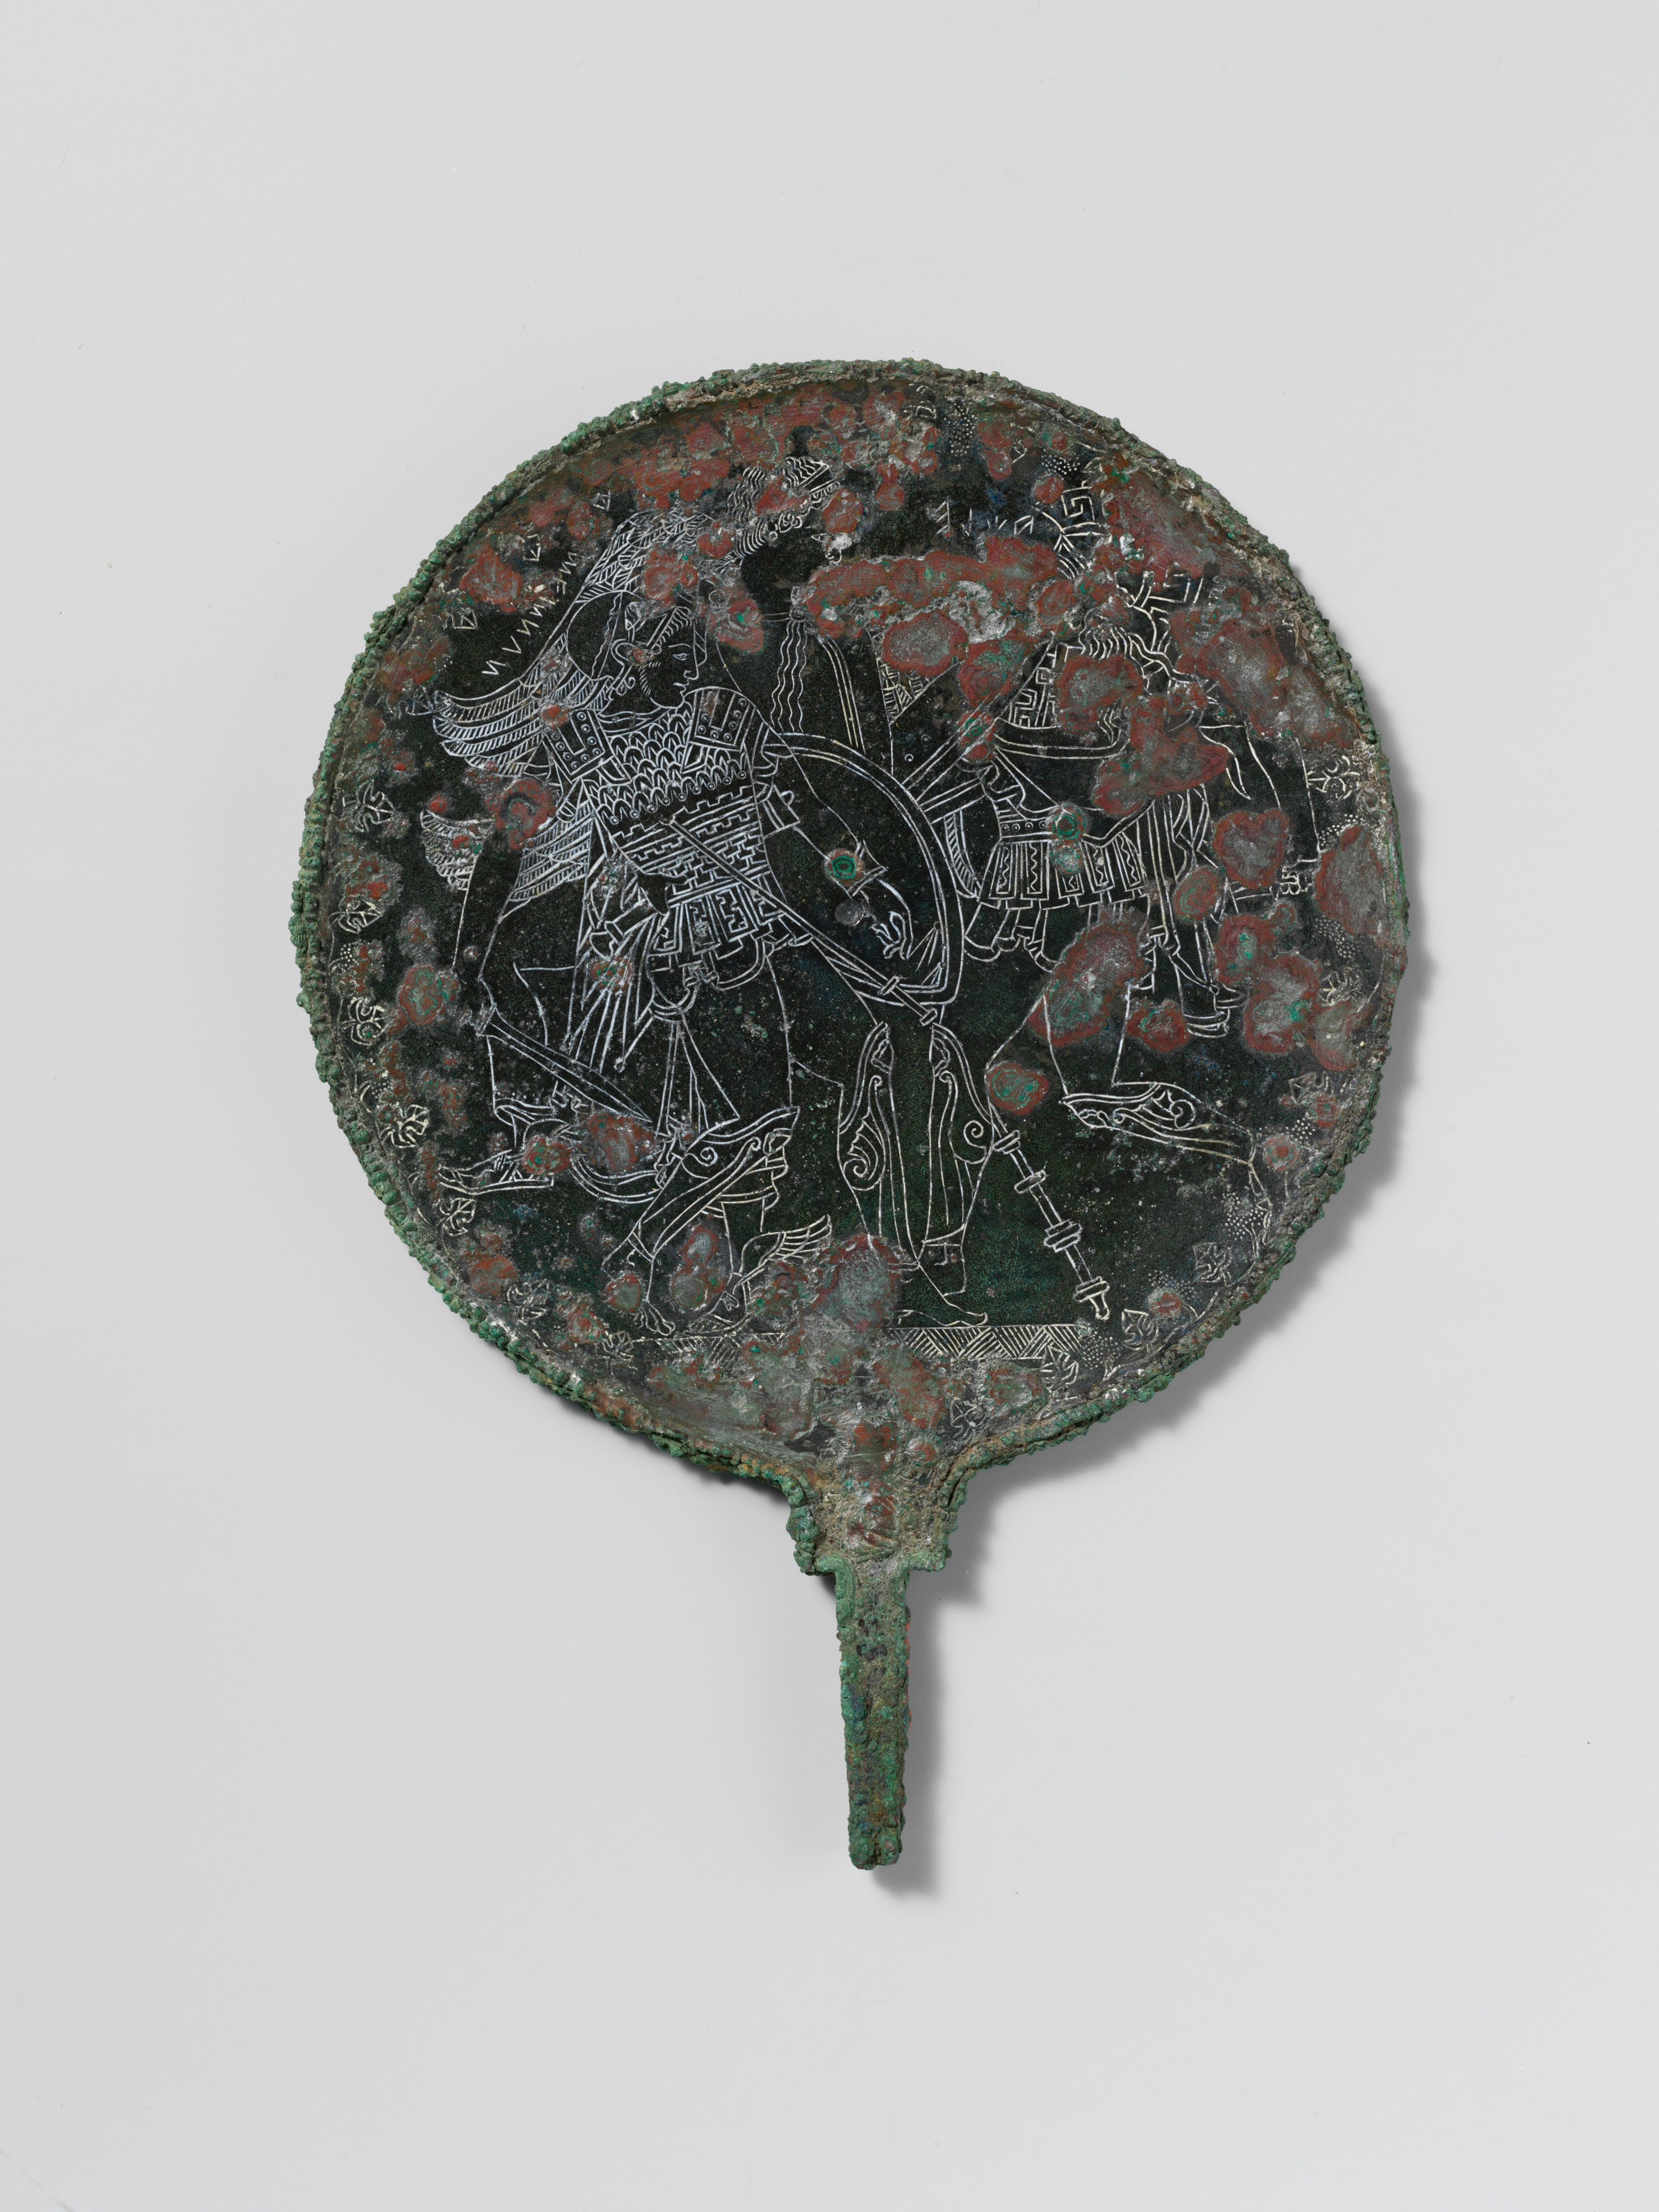
\includegraphics[width=0.45\linewidth]{met-bronze-mirror-22-139-84.jpg}
\caption{Bronze mirror, ca.\ 450--420 BCE. The Met, 22.139.84.}
\label{fig:mirror}
\end{figure}
Image: The Metropolitan Museum of Art. Public domain (CC0).
\end{document}
